\documentclass[tikz]{standalone}
\usepackage[utf8]{inputenx}%  http://ctan.org/pkg/inputenx
% Euler for math | Palatino for rm | Helvetica for ss | Courier for tt
\renewcommand{\rmdefault}{ppl}% rm
\linespread{1.025}% Palatino needs more leading
\usepackage[sc,osf]{mathpazo}
\usepackage[euler-digits,small]{eulervm}  %  http://ctan.org/pkg/eulervm
% a better implementation of the euler package (not in gwTeX)
\normalfont%
\usepackage[T1]{fontenc}%  http://ctan.org/pkg/fontenc
\usepackage{textcomp}%  http://ctan.org/pkg/textcomp
\begin{document}
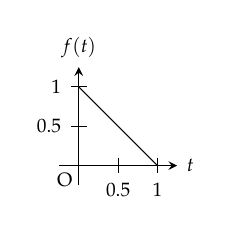
\begin{tikzpicture}
  % draw axis
  \draw[-stealth] (-0.25cm, 0) -- ++(1.5cm, 0) node[right, font = \scriptsize]
  {\(t\)};
  \draw[-stealth] (0, -0.25cm) -- ++(0, 1.5cm) node[above, font = \scriptsize]
  {\(f(t)\)};
  \node[font = \scriptsize] at (-135:0.25cm) {O};
  % draw tic marks for 1 on both axis
  \foreach \n in {0.5,1}{
    \draw (\n cm, 0.1cm) -- ++(0, -0.2cm) node[font = \scriptsize, below]
    {\(\n\)};
    \draw (0.1cm, \n cm) -- ++(-0.2cm, 0) node[font = \scriptsize, left]
    {\(\n\)};
  }
  % draw slope
  \draw (0, 1cm) -- (1cm, 0);
\end{tikzpicture}
\end{document}
%%% Local Variables:
%%% mode: latex
%%% TeX-master: t
%%% End:
